\documentclass[10pt,a4paper]{article}
\usepackage[utf8]{inputenc}
\usepackage{amsmath}
\usepackage{amsfonts}
\usepackage{amssymb}
\usepackage{float}
\usepackage{graphicx}
\usepackage[left=2cm,right=2cm,top=2cm,bottom=2cm]{geometry}
\usepackage{parskip}
\author{Songtuan Lin u6162630}
\title{Assignment 2}
\begin{document}
\maketitle
\section*{Question 1}
According to the definition of norm, the equation $\| \mathbf{x} - \mathbf{x_{0}} \|_{2} \leq \| \mathbf{x} - \mathbf{x_{1}} \|_{2}$ is the same as:
\begin{equation*}
	(\mathbf{x} - \mathbf{x_{0}})^{T} (\mathbf{x} - \mathbf{x_{0}}) \leq (\mathbf{x} - \mathbf{x_{1}})^{T} (\mathbf{x} - \mathbf{x_{1}})
\end{equation*}
Which can be further expressed as:
\begin{equation}
	\mathbf{x}^{T} (\mathbf{x_{1}} - \mathbf{x_{0}}) + (\mathbf{x_{1}} - \mathbf{x_{0}})^{T} \mathbf{x} \leq \mathbf{x_{1}}^{T} \mathbf{x_{1}} - \mathbf{x_{0}}^{T} \mathbf{x_{0}}
	\label{1}
\end{equation}
Since $\mathbf{x}^{T} (\mathbf{x_{1}} - \mathbf{x_{0}}) = \big( (\mathbf{x_{1}} - \mathbf{x_{0}})^{T} \mathbf{x} \big)^{T}$, which produce a constant, we have:
\begin{equation}
	\mathbf{x}^{T} (\mathbf{x_{1}} - \mathbf{x_{0}}) = (\mathbf{x_{1}} - \mathbf{x_{0}})^{T} \mathbf{x}
	\label{2}
\end{equation} 
Replace equation \ref{2} to equation \ref{1}, there is:
\begin{equation*}
	2 (\mathbf{x_{1}} - \mathbf{x_{0}})^{T} \mathbf{x} \leq \mathbf{x_{1}}^{T} \mathbf{x_{1}} - \mathbf{x_{0}}^{T} \mathbf{x_{0}}
\end{equation*}
Which follow the definition of half-space: $\mathbf{\lambda}^{T} \mathbf{x} \leq \mathbf{b}$, where $\mathbf{\lambda} = 2 (\mathbf{x_{1}} - \mathbf{x_{0}})$ and $\mathbf{b} = \mathbf{x_{1}}^{T} \mathbf{x_{1}} - \mathbf{x_{0}}^{T} \mathbf{x_{0}}$.

\section*{Question 2}
The polyhedron constructed by the convex hull is the area with the 5 color line as boundary, shown in following figure:
\begin{figure}[H]
	\begin{center}
		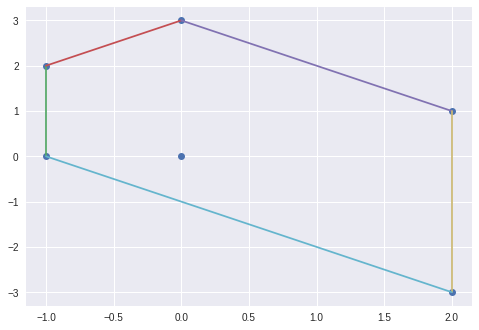
\includegraphics[scale=0.4]{Q2.png}
	\end{center}
\end{figure}
Denote $\mathbf{x} = \begin{bmatrix}
x_{1} \\
x_{2}
\end{bmatrix}$ as the point within $\mathcal{R}^{2}$, the hyper-plane defined by the 5 color line shown in above figure are:
\begin{equation*}
	\begin{bmatrix}
		-1 & 0 \\
		1 & 1 \\
		1 & 0 \\
		1 & 1
	\end{bmatrix} \mathbf{x} = 
	\begin{bmatrix}
		-1 \\
		-1 \\
		2 \\
		3
	\end{bmatrix}
\end{equation*}
As a result, the polyhedron constructed by these hyper-plane can be expressed as:
\begin{equation*}
	\mathcal{A} \mathbf{x} \preceq \mathbf{b}
\end{equation*}
Where $\mathcal{A} = \begin{bmatrix}
1 & 0 \\
1 & 1 \\
1 & 0 \\
1 & 1
\end{bmatrix}$ and $\mathbf{b} = \begin{bmatrix}
-1 \\
-1 \\
2 \\
3
\end{bmatrix}$

\section*{Question 3}

\subsection*{(a)}
Denote set $\{ \mathbf{x} |\, \alpha \leq \mathbf{a}^{T}\mathbf{x} \leq \beta \}$ as $\mathcal{C}$, then, $\mathcal{C}$ is a convex set. The prove is as follow:

Assume $\mathbf{x_{1}}, \mathbf{x_{2}} \in \mathcal{C}$, their convex combination follow:
\begin{equation}
	\mathbf{a}^{T}(\theta \mathbf{x_{1}} + (1 - \theta) \mathbf{x_{2}}) = \theta \mathbf{a}^{T} \mathbf{x} + (1 - \theta) \mathbf{a}^{T} \mathbf{x_{2}}
	\label{3}
\end{equation}
Since $\mathbf{x_{1}}, \mathbf{x_{2}} \in \mathcal{C}$, there is:
\begin{equation}
	\begin{cases}
		\mathbf{a}^{T} \mathbf{x_{1}} \geq \alpha \\
		\mathbf{a}^{T} \mathbf{x_{2}} \geq \alpha
	\end{cases}
	\label{4}
\end{equation}
Combine equation \ref{3} and \ref{4}, we have:
\begin{align*}
	\theta \mathbf{a}^{T} \mathbf{x} + (1 - \theta) \mathbf{a}^{T} \mathbf{x_{2}} &\geq \theta \alpha + (1 - \theta) \alpha \\
	&= \alpha
\end{align*}
The equation $\theta \mathbf{a}^{T} \mathbf{x} + (1 - \theta) \mathbf{a}^{T} \mathbf{x_{2}} \leq \beta$ can be proved by using the same method. As a result, when $\mathbf{x_{1}}, \mathbf{x_{2}} \in \mathcal{C}$, $\theta \mathbf{x_{1}} + (1 - \theta) \mathbf{x_{2}} \in \mathcal{C}$ hold for any $0 \leq \theta \leq 1$. Thus, $\mathcal{C}$ is a convex set.

\subsection*{(b)}
The \textit{rectangle} set $\mathcal{G}$ can be thought as the intersection of different sets that follow:
\begin{equation*}
	\mathcal{G} = \displaystyle\bigcap_{i = 1}^{n} \mathcal{G}_{i}
\end{equation*}
Where $\mathcal{G}_{i}$ is the set: $\{ \mathbf{x} |\, \alpha \leq x_{i} \leq \beta \}$. It is obvious that $\mathcal{G}_{i}$ is the \textit{slab} defined in (a) with 
\begin{equation*}
	\mathbf{a} = 
	\begin{bmatrix}
		0 \\
		\vdots \\
		1 \\
		\vdots \\
		0
	\end{bmatrix}
\end{equation*}
In which, the ith element $a_{i}$ that corresponding to $x_{i}$ within $\mathbf{x}$ is set to be 1 and the other elements is 0. Therefore, $\mathcal{G}_{i}$ is convex, which means, $\mathcal{G}$ is the intersection of convex set, which is also convex. 

\subsection*{(c)}
The set $\{ \mathbf{x} |\, \mathbf{a_{1}}^{T} \mathbf{x} \leq b_{1}, \mathbf{a_{2}}^{T} \mathbf{x} \leq b_{2} \}$ is the same as:
\begin{equation*}
\{ \mathbf{x} |\, \mathbf{a_{1}}^{T} \mathbf{x} \leq b_{1} \} \cap \{ \mathbf{x} |\, \mathbf{a_{2}}^{T} \mathbf{x} \leq b_{2} \}
\end{equation*}
For any $i \in \{ 0, 1 \}$, the set $\{ \mathbf{x} |\, \mathbf{a_{i}}^{T} \mathbf{x} \leq b_{i} \}$ define a half-space, which is a convex set. As a result, the set $\{ \mathbf{x} |\, \mathbf{a_{1}}^{T} \mathbf{x} \leq b_{1}, \mathbf{a_{2}}^{T} \mathbf{x} \leq b_{2} \}$ is the intersection of two convex set, which is also convex.

\subsection*{(d)}
Assume $\mathcal{S} = \{ \mathbf{s_{1}}, \mathbf{s_{2}}, \cdots, \mathbf{s_{n}} \}$. The original set $\{ \mathbf{x} |\, \| \mathbf{x} - \mathbf{x_{0}} \|_{2} \leq \| \mathbf{x} - \mathbf{s} \|_{2} \text{ for any } \mathbf{s} \in \mathcal{S} \}$ can be expressed as:
\begin{equation*}
	\displaystyle\bigcap_{i = 1}^{n}\{ \mathbf{x} |\, \| \mathbf{x} - \mathbf{x_{0}} \|_{2} \leq \| \mathbf{x} - \mathbf{s_{i}} \|_{2} \}
\end{equation*}
The same concept can be expanded to set $\mathcal{S}$ which has infinite element($n \rightarrow \infty$). According to Question 1, the single set $\mathbf{x} |\, \| \mathbf{x} - \mathbf{x_{0}} \|_{2} \leq \| \mathbf{x} - \mathbf{s_{i}} \|_{2}$ define a half-space and is convex. As a result, the intersection of these convex is also convex, which means, $\{ \mathbf{x} |\, \| \mathbf{x} - \mathbf{x_{0}} \|_{2} \leq \| \mathbf{x} - \mathbf{s} \|_{2} \text{ for any } \mathbf{s} \in \mathcal{S} \}$ is convex.

\subsection*{(e)}
We first consider the set:
\begin{equation}
	\mathcal{G}_{i} = \{ \mathbf{x} |\, \| \mathbf{x} - \mathbf{s_{i}} \|_{2} \leq \| \mathbf{x} - \mathbf{s} \|_{2} \textit{ for all } \mathbf{s} \in \mathcal{S} \}
	\label{5}
\end{equation}
Where $\mathbf{s_{i}} \in \mathcal{S}$ is a fixed point within $\mathcal{S}$. This set is consist of points $\mathbf{x}$ that have the minimum distance to $\mathcal{S}$ through $\mathbf{s_{i}}$. It is obvious that
\begin{equation}
	\{ \mathbf{x} |\, \| \mathbf{x} - \mathbf{s_{i}} \|_{2} \leq \| \mathbf{x} - \mathbf{s} \|_{2} \} \cap \{ \mathbf{x} |\, \| \mathbf{x} - \mathbf{s_{j}} \|_{2} \leq \| \mathbf{x} - \mathbf{s} \|_{2} \} = \emptyset
	\label{6}
\end{equation}
when $\mathbf{s_{i}}, \mathbf{s_{j}} \in \mathcal{S}$ and $\mathbf{s_{i}} \neq \mathbf{s_{j}}$ as a point $\mathbf{x}$ can only achieve the minimum distance to $\mathcal{S}$ by hold $\| \mathbf{x} - \mathbf{s_{i}} \| < \| \mathbf{x} - \mathbf{s_{j}} \|$ or the inverse. Now assume $\mathcal{S} = \{ \mathbf{s_{1}}, \mathbf{s_{2}}, \cdots, \mathbf{s_{n}} \}$ and $\mathcal{T} = \{ \mathbf{t_{1}}, \mathbf{t_{2}}, \cdots, \mathbf{t_{k}} \}$. We define the set:
\begin{equation*}
	\mathcal{Q}_{i} = \{ \mathbf{x} |\, \| \mathbf{x} - \mathbf{s_{i}} \|_{2} \leq \| \mathbf{x} - \mathbf{t} \|_{2} \textit{ for all } \mathbf{t} \in \mathcal{T} \}
\end{equation*}
Where $\mathbf{s_{i}} \in \mathcal{S}$. This set describe the point $\mathbf{x}$ that the distance between $\mathbf{x}$ and a point $\mathbf{s_{i}} \in \mathcal{S}$ is less than the distance between $\mathbf{x}$ and set $\mathcal{T}$. As a result, the set $\{ \mathbf{x} |\, \textbf{dist}(\mathbf{x}, \mathcal{S}) < \textbf{dist}(\mathbf{x}, \mathcal{T}) \}$ can be then expressed as:
\begin{equation*}
	\displaystyle\bigcup_{i = 1}^{n}(\mathcal{G}_{i} \cap \mathcal{Q}_{i})
\end{equation*}
According to equation \ref{6}, for any $1 \leq i, j \leq n$, $\mathcal{G}_{i} \cap \mathcal{G}_{j} = \emptyset$. Hence, $(\mathcal{G}_{i} \cap \mathcal{Q}_{i}) \cup (\mathcal{G}_{j} \cap \mathcal{Q}_{j}) = \emptyset$, which means, the set $\{ \mathbf{x} |\, \textbf{dist}(\mathbf{x}, \mathcal{S}) < \textbf{dist}(\mathbf{x}, \mathcal{T}) \}$  is separated and therefore can not be convex.

\subsection*{(f)}
Assume $\mathcal{S}_{1} = \{ \mathbf{s_{1}}, \mathbf{s_{2}}, \cdots, \mathbf{s_{n}} \}$. Then, the set $\mathcal{C} =  \{ \mathbf{x} |\, \mathbf{x} + \mathcal{S}_{1} \subset \mathcal{S}_{2} \}$ can be replaced as the intersection of different set as:
\begin{equation*}
	\mathcal{C} = \displaystyle\bigcap_{i = 1}^{n}\mathcal{C}_{i}
\end{equation*}
Where $\mathcal{C}_{i} = \{ \mathbf{x} |\, \mathbf{x} + \mathbf{s_{i}} \in \mathcal{S}_{2} \}$. It can be proved that $\mathcal{C}_{i}$ is convex: Assume $\mathbf{x_{1}}, \mathbf{x_{2}} \in \mathcal{C}_{i}$. The equation $\theta \mathbf{x_{1}} + (1 - \theta) \mathbf{x_{2}} + \mathbf{s_{i}}$ can be expressed as:
\begin{equation*}
	\theta \mathbf{x_{1}} + (1 - \theta) \mathbf{x_{2}} + \mathbf{s_{i}} = \theta(\mathbf{x_{1}} + \mathbf{s_{i}})  + (1 - \theta) (\mathbf{x}_{2} + \mathbf{s_{i}})
\end{equation*}
Since $\mathbf{x_{1}} + \mathbf{s_{i}}, \mathbf{x_{2}} + \mathbf{s_{i}} \in \mathcal{S}_{2}$ and $\mathcal{S}_{2}$ is convex, we have $\theta(\mathbf{x_{1}} + \mathbf{s_{i}})  + (1 - \theta) (\mathbf{x}_{2} + \mathbf{s_{i}}) \in \mathcal{S}_{2}$. Hence, $\mathcal{C}_{i}$ is convex. As a result, $\mathcal{C}$ is convex as it is the intersection of convex set.

\subsection*{(g)}
The equation $\| \mathbf{x} - \mathbf{a} \|_{2} \leq \theta \| \mathbf{x} - \mathbf{b} \|_{2}$ is the same as $\| \mathbf{x} - \mathbf{a} \|^{2}_{2} \leq \theta^{2} \| \mathbf{x} - \mathbf{b} \|^{2}_{2}$. Now, let $\theta^{2} = p$, the equation mentioned before can be expanded as:
\begin{equation}
	\mathbf{x}^{T}\mathbf{x} + \frac{2 (p \mathbf{b} - \mathbf{a})^{T}}{1 - p} \mathbf{x} + \frac{\mathbf{a}^{T} \mathbf{a} - p \mathbf{b}^{T}\mathbf{b}}{1 - p} \leq 0
	\label{7}
\end{equation}
Which has the same form as the equation that describe a ball:
\begin{equation}
	\| \mathbf{x} - \mathbf{x_{0}} \|^{2}_{2} = \mathbf{x}^{T} \mathbf{x} - 2 \mathbf{x_{0}}^{T} \mathbf{x} + \mathbf{x_{0}}^{T} \mathbf{x_{0}} \leq r^{2}
	\label{8}
\end{equation}
Compare equation \ref{7} with \ref{8}, it is easy to figure out that:
\begin{equation*}
	\mathbf{x_{0}} = \frac{\mathbf{a} - p \mathbf{b}}{1 - p} \textit{ and } r^{2} = \mathbf{x_{0}}^{T} \mathbf{x_{0}} - \frac{\mathbf{a}^{T} \mathbf{a} - p \mathbf{b}^{T} \mathbf{b}}{1 - p}
\end{equation*}
If $r^{2} \geq 0 $ can be verified, then, equation \ref{7} always describe a ball. Indeed, $r^{2}$ can be expanded as:
\begin{equation*}
	r^{2} = \frac{(\mathbf{a} - p \mathbf{b})^{T} (\mathbf{a} - p \mathbf{b})}{(1 - p)^{2}} - \frac{\mathbf{a}^{T} \mathbf{a} - p \mathbf{b}^{T} \mathbf{b}}{1 - p}
\end{equation*}
Which is the same as:
\begin{equation*}
	r^{2} = \frac{p(\mathbf{a}^{T} \mathbf{a} - 2 \mathbf{a}^{T} \mathbf{b} + \mathbf{b}^{T} \mathbf{b})}{(1 - p)^{2}}
\end{equation*}
Since $\mathbf{a}^{T} \mathbf{a} - 2 \mathbf{a}^{T}\mathbf{b} + \mathbf{b}^{T} \mathbf{b} = \| \mathbf{a} - \mathbf{b} \|^{2}_{2} \geq 0$, $r^{2}$ is also greater or equal to zero. Hence, equation \ref{7} describe a ball, which is a convex set.

\section*{Question 4}
In this question, we firstly define the vector:
\begin{equation}
	\mathbf{x} = \begin{bmatrix}
	a_{0} \\
	a_{1} \\
	\vdots \\
	a_{n}
	\end{bmatrix}
	\label{9}
\end{equation}
Which contain all possible value that random variable $x$ may take. After that, the vector $\mathbf{p}$ which describe the probability distribution of $x$:
\begin{equation}
	\mathbf{p} = \begin{bmatrix}
	p_{1} \\
	p_{2} \\
	\vdots \\
	p_{n}
	\end{bmatrix}
	\label{10}
\end{equation}
Where the element $p_{i}$ within $\mathbf{p}$ corresponding to the probability that $x = a_{i}$. It is obvious that the set $\mathcal{P} = \{ \mathbf{p} |\, \| \mathbf{p} \| = 1 \textit{ and for each } p_{i} \textit{ within } \mathbf{p}, p_{i} \geq 0 \}$ is a convex set.

\subsection*{(a)}
Follow the definition used in \ref{9} and \ref{10}, we can define vector $\mathbf{f}$ as:
\begin{equation*}
	\mathbf{f} = \begin{bmatrix}
	f(a_{1}) \\
	f(a_{2}) \\
	\vdots \\
	f(a_{n})
	\end{bmatrix}
\end{equation*}
The condition $\alpha \leq \mathcal{E}f(x) \leq \beta$ define a set $\mathcal{Q}$ which is a intersection of two half-space:
\begin{equation*}
	\mathcal{Q} = \{ \mathbf{p} |\, -\mathbf{f}^{T} \mathbf{p} \leq -\alpha \} \cap \{ \mathbf{p} |\, \mathbf{f}^{T} \mathbf{p} \leq \beta \}
\end{equation*}
As a result, the set of $\mathbf{p}$ that satisfied the condition $\alpha \leq \mathcal{E}f(x) \leq \beta$ is the intersection of $\mathcal{P}$ and $\mathcal{Q}$, which produce a convex set.

\subsection*{(b)}
We firstly define a indicator vector $\mathbf{i}$ as:
\begin{equation*}
	\mathbf{i} = \begin{bmatrix}
	\mathbb{I}(a_{1} > \alpha) \\
	\mathbb{I}(a_{2} > \alpha) \\
	\vdots \\
	\mathbb{I}(a_{n} > \alpha)
	\end{bmatrix}
\end{equation*}
Where $\mathbb{I}(s)$ is defined as:
\begin{equation*}
	\mathbb{I}(s) = 
	\begin{cases}
		1 & \quad \textit{if } s \textit{ is true} \\
		0 & \quad \textit{otherwise}
	\end{cases}
\end{equation*} 
Therefore, the constrain can be expressed as:
\begin{equation*}
	\mathbf{i}^{T} \mathbf{p} \leq \beta
\end{equation*}
Which obviously, define a half-space. Therefore, the set defined by this half-space: $\mathcal{Q} = \{ \mathbf{p} |\,  \mathbf{i}^{T} \mathbf{p} \leq \beta \}$ is a convex set. Consequently, the set of $\mathbf{p}$ that satisfied the constrain can be expressed as $\mathcal{P} \cap \mathcal{Q}$, which is convex.

\subsection*{(c)}
Let $f(x)$ in (a) equal to $x^{2}$. Hence, there is:
\begin{equation*}
	\mathbf{f} = \begin{bmatrix}
	a_{1}^{2} \\
	a_{2}^{2} \\
	\vdots \\
	a_{n}^{2}
	\end{bmatrix}
\end{equation*}
The constrain $\mathcal{E}x^{2} \geq \alpha$ can then be expressed as:
\begin{equation*}
	-\mathbf{f}^{T} \mathbf{p} \leq -\alpha
\end{equation*}
Which define a half-space. Hence, the set of $\mathbf{p}$ under this constrain is convex.

\subsection*{(d)}
Assume $\mathbf{x} = \begin{bmatrix}
1 \\
0
\end{bmatrix}$, $\mathbf{p_{1}} = \begin{bmatrix}
1 \\
0
\end{bmatrix}$ and $\mathbf{p_{2}} = \begin{bmatrix}
0 \\
1
\end{bmatrix}$. Set $\alpha = 0.2$. Therefore, for $\mathbf{p_{1}}$, we have:
\begin{equation*}
	Var(\mathbf{x}) = 0 < 0.2
\end{equation*}
For $\mathbf{p_{2}}$, we have:
\begin{equation*}
	Var(\mathbf{x}) = 0 < 0.2
\end{equation*}
However, for $\mathbf{p_{3}} = 0.5 \mathbf{p_{1}} + 0.5 \mathbf{p_{2}}$, there is:
\begin{equation*}
	Var(\mathbf{x}) = 0.25 > 0.2
\end{equation*}
Hence, the set of $\mathbf{p}$ that satisfied this constrain is not convex.

\section*{Question 5}
\subsection*{(a)}
As the function $f(\mathbf{x}, \mathbf{z})$ is convex over $\mathbf{x}$, it's Hessian Matrix over $\mathbf{x}$ is:
\begin{equation*}
	\mathcal{H}_{\mathbf{x}} = \begin{bmatrix}
	\frac{\partial^{2} f}{\partial x_{1}^{2}} & \frac{\partial^{2} f}{\partial x_{1} x_{2}} & \cdots & \frac{\partial^{2} f}{\partial x_{1} x_{n}} \\
	\frac{\partial^{2} f}{\partial x_{2} x_{1}} & \frac{\partial^{2} f}{\partial x_{2}^{2}} & \cdots & \frac{\partial^{2} f}{\partial x_{2} x_{n}} \\
	\vdots & \vdots & \ddots & \vdots \\
	\frac{\partial^{2} f}{\partial x_{n} x_{1}} & \frac{\partial^{2} f}{\partial x_{n} x_{2}} & \cdots & \frac{\partial^{2} f}{\partial x_{n}^{2}}
	\end{bmatrix}
\end{equation*}
Which satisfied $\mathcal{H}_{\mathbf{x}} \succeq 0$. The Hessian Matrix of $f$ over $\mathbf{z}$: $\mathcal{H}_{\mathbf{z}}$ has the similar form as $\mathcal{H}_{\mathbf{x}}$ and satisfied: $\mathcal{H}_{\mathbf{z}} \preceq 0$. As a result, the Hessian Matrix over $\mathbf{x}$ and $\mathbf{z}$ should be:
\begin{equation*}
	\nabla^{2} f(\mathbf{x}, \mathbf{z}) = \begin{bmatrix}
	\mathcal{H}_{\mathbf{x}} & \mathcal{H}_{\mathbf{z}} \\
	\mathcal{H}_{\mathbf{z}} & \mathcal{H}_{\mathbf{x}}
	\end{bmatrix}
\end{equation*}

\subsection*{(b)}
Firstly, we fix $\mathbf{x} = \tilde{\mathbf{x}}$. Since $f$ is concave over $\mathbf{z}$ and $\nabla f(\tilde{\mathbf{x}}, \tilde{\mathbf{z}}) = 0$, according to the first-order condition of concave function, we have, for any $\mathbf{z}$:
\begin{equation}
	f(\tilde{\mathbf{x}}, \mathbf{z}) < f(\tilde{\mathbf{x}}, \tilde{\mathbf{z}})
	\label{11}
\end{equation}
In order to prove $f(\tilde{\mathbf{x}}, \tilde{\mathbf{z}}) < f(\mathbf{x}, \tilde{\mathbf{z}})$. We fix $\mathbf{z} = \tilde{\mathbf{z}}$. Since $f$ is convex over $\mathbf{x}$, according to the first-order condition of convex function, there is:
\begin{equation*}
	f(\tilde{\mathbf{x}}, \tilde{\mathbf{z}}) + \nabla f(\tilde{\mathbf{x}}, \tilde{\mathbf{z}}) (\mathbf{x} - \tilde{\mathbf{x}}) < f(\mathbf{x}, \tilde{\mathbf{z}})
\end{equation*}
Since $\nabla f(\tilde{\mathbf{x}}, \tilde{\mathbf{z}}) = 0$, we can prove that:
\begin{equation*}
	f(\tilde{\mathbf{x}}, \tilde{\mathbf{z}}) < f(\mathbf{x}, \tilde{\mathbf{z}})
\end{equation*}

Then, we start to prove $\displaystyle\sup_{\mathbf{z}} \displaystyle\inf_{\mathbf{x}}f(\mathbf{x}, \mathbf{z}) = f(\tilde{\mathbf{x}}, \tilde{\mathbf{z}})$: For any $\mathbf{z}$, if $\displaystyle\inf_{\mathbf{x}}f(\mathbf{x}, \mathbf{z}) = f(\mathbf{x}^{*}, \mathbf{z})$, we have:
\begin{equation*}
	f(\mathbf{x}^{*}, \mathbf{z}) \leq f(\tilde{\mathbf{x}}, \mathbf{z})
\end{equation*}
Which means, $\displaystyle\inf_{\mathbf{x}}f(\mathbf{x}, \mathbf{z}) \leq f(\tilde{\mathbf{x}}, \mathbf{z})$. The equality hold when $\mathbf{x}^{*} = \tilde{\mathbf{x}}$. Furthermore, according to equation \ref{11}, $\tilde{\mathbf{z}}$ maximize $f(\tilde{\mathbf{x}}, \mathbf{z})$ over $\mathbf{z}$. Therefore, we can conclude that the infimum of $f(\mathbf{x}, \mathbf{z})$ is smaller than or equal to $f(\tilde{\mathbf{x}}, \mathbf{z})$, which has the maximum value $f(\tilde{\mathbf{x}}, \tilde{\mathbf{z}})$.This conclusion is the same as:
\begin{equation*}
	\displaystyle\sup_{\mathbf{z}}\inf_{\mathbf{x}} = f(\tilde{\mathbf{x}}, \tilde{\mathbf{z}})
\end{equation*}
The similar method can be used to prove:
\begin{equation*}
	\displaystyle\inf_{\mathbf{x}}\sup_{\mathbf{z}} = f(\tilde{\mathbf{x}}, \tilde{\mathbf{z}})
\end{equation*}
Hence, $\displaystyle\sup_{\mathbf{z}}\inf_{\mathbf{x}} = \displaystyle\inf_{\mathbf{x}}\sup_{\mathbf{z}} = f(\tilde{\mathbf{x}}, \tilde{\mathbf{z}})$

\subsection*{(c)}
We firstly fix $\mathbf{x} = \tilde{\mathbf{x}}$. According to $f(\tilde{\mathbf{x}}, \mathbf{z}) \leq f(\tilde{\mathbf{x}}, \tilde{\mathbf{z}})$, $f(\tilde{\mathbf{x}}, \tilde{\mathbf{z}})$ is the maximum value of function $f(\tilde{\mathbf{x}}, \mathbf{z})$ over $\mathbf{z}$. Hence, there is:
\begin{equation*}
	\nabla_{\mathbf{x}} f(\tilde{\mathbf{x}}, \tilde{\mathbf{z}}) = 0
\end{equation*}
Furthermore, we can identify that $f(\tilde{\mathbf{x}}, \tilde{\mathbf{z}})$ is the minimum of $f(\mathbf{x}, \tilde{\mathbf{z}})$ over $\mathbf{x}$ when we fix $\mathbf{z} = \tilde{\mathbf{z}}$, there is:
\begin{equation*}
	\nabla_{\mathbf{z}} f(\tilde{\mathbf{x}}, \tilde{\mathbf{z}}) = 0
\end{equation*}
Combine the above two equation, we have: $\nabla f(\tilde{\mathbf{x}}, \tilde{\mathbf{z}}) = 0$

\section*{Question 6}
\subsection*{(a)}
This function is convex and quasi-convex. Furthermore, this function is also quasi-concave but not concave.
\subsection*{(b)}
This function is neither convex nor concave as it's Hessian Matrix is not semi-definite or negative semi-definite. However, this function is quasi-convex but not quasi-concave.
\subsection*{(c)}
This function is convex and quasi-convex as it's Hessian Matrix is semi-definite. This function is neither concave nor quasi-concave.
\subsection*{(d)}
This function is neither convex nor concave. However, this function is both quasi-convex and quasi-concave.
\subsection*{(e)}
This function is convex and quasi-convex but not concave and quasi-concave.
\subsection*{(f)}
This function is concave and quasi-concave but not convex and quasi-convex.

\section*{Question 7}
\subsection*{(a)}
The conjugate function of $f(\mathbf{x})$ is:
\begin{equation*}
	f^{*}(\mathbf{y}) = 
	\begin{cases}
		0 \quad \textit{if } \mathbf{1}^{T} \mathbf{y} = 1 \textit{ and } \mathbf{y} \succeq 0  \\
		\infty \quad \textit{otherwise}
	\end{cases}
\end{equation*}
Firstly, we verify the domain: $\textbf{dom}f^{*}(\mathbf{y})$ is $\mathbf{y} \succeq 0$ and $\mathbf{1}^{T} \mathbf{y} = 1$: if $y_{k}$ within $\mathbf{y}$ is negative, then, for $\mathbf{x}$ that satisfied: $x_{k} \rightarrow \infty$ and $x_{i} = 0$ for any $i \neq k$, there is:
\begin{equation*}
	\mathbf{y}^{T} \mathbf{x} - max(\mathbf{x}) \rightarrow -\infty
\end{equation*}
Hence, $\mathbf{y}$ with negative components is not in the $\textbf{dom}f^{*}$. Then, we prove when $\mathbf{1}^{T} \mathbf{y} \neq 1$, $\mathbf{y}$ is not in the domain of $f^{*}$. This can be easily verified by setting $n = 1$: Assume $y = q > 1$, we have $f^{*}(q) = \displaystyle\sup_{x}(q - 1)x$, which goes to infinity when $x \rightarrow \infty$. Besides, when $y = p < 1$, $f^{*}(p)$ goes to infinity when $x \rightarrow -\infty$. As a result, $y$ must equal to 1.

When $\mathbf{1}^{T} \mathbf{y} = 1$ and $\mathbf{y} \succeq 0$, $\mathbf{y}^{T} \mathbf{x}$ is the convex combination of elements within $\mathbf{x}$. Hence, $max(\mathbf{y}^{T} \mathbf{x}) = max(\mathbf{x})$, which means:
\begin{equation*}
	\displaystyle\sup_{\mathbf{x}}(\mathbf{y}^{T} \mathbf{x} - max(\mathbf{x})) = 0
\end{equation*} 
\subsection*{(b)}
As what we do in (a), we firstly define the domain of $f^{*}(\mathbf{y})$. Assume there is negative component $y_{i} < 0$ within $\mathbf{y}$. For such $\mathbf{y}$, we can find a $\mathbf{x}$, in which $x_{i} = t$ and $x_{j} = 0$ when $i \neq j$. As a result, the conjugate function become:
\begin{equation*}
	f^{*}(\mathbf{y}) = \displaystyle\sup_{\mathbf{x}}(y_{i} x_{i} - x_{i})
\end{equation*}
Which goes to infinity when $t \rightarrow \infty$. As a result, $\mathbf{y} \succeq 0$. Furthermore

\end{document}